%----------------------------------------------------------------------------------------
%	PACKAGES AND THEMES (LMU beamer template)
%----------------------------------------------------------------------------------------

\documentclass[aspectratio=169]{beamer}
\mode<presentation> {
	\usetheme{Boadilla}
}
\definecolor{lmugreen}{RGB}{0, 136, 58}
\usecolortheme[named=lmugreen]{structure}
\usepackage{graphicx} % Allows including images
\usepackage{booktabs} % Allows the use of \toprule, \midrule and \bottomrule in tables
\usepackage[english]{babel}
\usepackage[utf8]{inputenc}
\usepackage{amsmath,amssymb} % math symbols
\usepackage{float}
\usepackage{hyperref} % for URLs
\newcommand{\gray}{\rowcolor[gray]{.90}}
\usepackage{verbatim}
\usepackage{textpos} % logo position
% Font of the template. Loaded only when the TeX installation has it.
\IfFileExists{sourcesanspro.sty}{\usepackage[default]{sourcesanspro}}{}
\usepackage{cases} % math cases

% Citations follow the thesis: natbib with round brackets and commas.
\usepackage[round, comma]{natbib}

% Frame numbers restart after \appendix, so the main talk shows its own total.
\IfFileExists{appendixnumberbeamer.sty}{\usepackage{appendixnumberbeamer}}{}

% Caption
\usepackage{caption}
\DeclareCaptionFont{tiny}{\tiny}
\captionsetup{font=scriptsize,labelfont=scriptsize,justification=centering}

% ToC. One outline frame at the start of each section.
\AtBeginSection[]{
	\begin{frame}[noframenumbering, plain]
	\frametitle{Outline}
	\setcounter{tocdepth}{1}
	\tableofcontents[currentsection]
\end{frame}
}

% Remove navigation
\beamertemplatenavigationsymbolsempty

%----------------------------------------------------------------------------------------
%	TITLE DATA
%----------------------------------------------------------------------------------------

\newcommand{\mytitle}{Evidential Bayesian Neural Networks for Uncertainty-Aware Classification}
\newcommand{\myshorttitle}{Evidential Bayesian Neural Networks}
\newcommand{\myname}{John-Pierre Weideman}
\newcommand{\mydate}{TODO: defence date}

\addtobeamertemplate{frametitle}{}{%
	\begin{textblock*}{100mm}(0.88\textwidth,-0.5cm)
		
\includegraphics[height=1cm,width=2cm]{lmu_logo}
\end{textblock*}}

\title[\myshorttitle]{\mytitle}
\author{\myname}
\institute[LMU]{Department of Statistics, LMU Munich}
\date{\mydate}

\begin{document}

% Content helpers. The LMU template preamble is unchanged.
% \textbf{TODO: Add the defence date when the author supplies it.}
\renewcommand{\mydate}{}
% Use native Beamer lists so subitems retain the template's smaller default style.
\newcommand{\slidepoint}[1]{\begin{itemize}\item #1\end{itemize}}
\newcommand{\slidemessage}[1]{\slidepoint{{\large #1}}\medskip}
\definecolor{introblue}{RGB}{50,106,159}
% Shared class legend for the introduction's mathematical illustrations.
\newcommand{\introlegend}[1][Two class illustration]{%
\begin{center}
\textcolor{lmugreen}{\rule{4mm}{3mm}}\ Class A\qquad
\textcolor{introblue}{\rule{4mm}{3mm}}\ Class B\qquad
#1
\end{center}}

\newcommand{\exampleindex}{4195}
\newcommand{\exampletotal}{52}
\newcommand{\examplecounts}{(0,0,0,29,0,23,0,0,0,0)}


%----------------------------------------------------------------------------------------
%	TITLE FRAME
%----------------------------------------------------------------------------------------

{
\usebackgroundtemplate{
\includegraphics[width=\paperwidth]{lmu-background.pdf}}
% Source. Thesis main.tex title page and Background 2.2, eq:dirichlet-density.
\begin{frame}[noframenumbering, plain]
\label{frm:title}
\begin{columns}[onlytextwidth]
	\begin{column}{0.38\textwidth}
		\vspace{2.5cm}

		\textbf{\textcolor{white}{\large \mytitle}}
		\vspace{1cm}

		\textcolor{white}{\footnotesize \myname \\
			\mydate}
	\end{column}
	\hfill
	\begin{column}{0.48\textwidth}
		\vspace{2cm}
		\begin{center}
			% Source. Background 2.2, eq:dirichlet-density. Illustration from scripts/build_figures.py.
			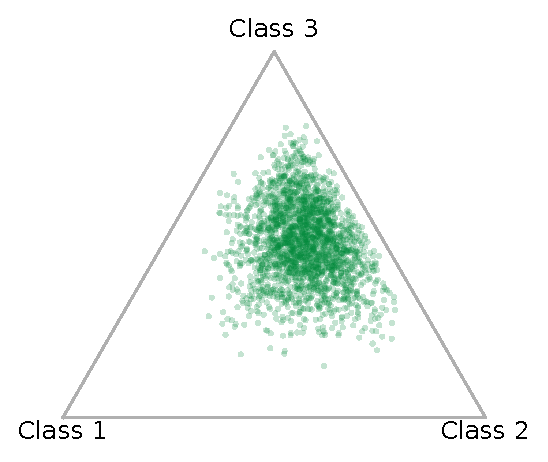
\includegraphics[width=1\textwidth]{figures/dirichlet_cover.pdf}
		\end{center}
	\end{column}
\end{columns}
\end{frame}
}

%----------------------------------------------------------------------------------------
%	SECTIONS. One file per section, see STORY.md.
%----------------------------------------------------------------------------------------

% Section 1. Introduction
% Goal. The examiners see the problem before they see a model. See STORY.md.

\section{Introduction}

% Slide 1.1. Source: Experiments 5.1.1 (sec:exp-setup, CIFAR-10H, peterson2019human).
% New figure from scripts/.
\begin{frame}{A Class Label Alone Is Not Enough}
	\textbf{Message.} Annotators disagree on some images. A model must say how sure it is, and why.

	\medskip
	\textbf{TODO: content.} One CIFAR-10H image with its count vector over the ten classes. One sentence on predictive uncertainty and its sources.
\end{frame}

% Slide 1.2. Source: Introduction. Background 2.7 (sec:bg-three-way-decomposition).
% malinin2018priornetworks.
\begin{frame}{Three Sources of Predictive Uncertainty}
	\textbf{Message.} Predictive uncertainty has three sources. Aleatoric, epistemic, and distributional uncertainty.

	\medskip
	\textbf{TODO: content.} Three rows. Name, one line definition, one intuition each. No equations.
\end{frame}

% Slide 1.3. Source: Introduction. Discussion 6.1 (sec:discussion-representation).
% sensoy2018edl, ulmer2023survey.
\begin{frame}{The Gap and Our Contribution}
	\textbf{Message.} Categorical BNNs represent two of the three terms. EDL represents two. We combine them into two models that represent all three.

	\medskip
	\textbf{TODO: content.} Table of models against uncertainty terms. Two lines. Cat-eBNN with one label per input and a prior. DM-eBNN with repeated labels. Spell out all acronyms.
\end{frame}

% Background. Model definitions prepare the contributions and their interpretation.
\section{Background}
% Source. Background 2.1, eq:class-probability-vector, eq:categorical-likelihood,
% eq:likelihood-factorization, eq:bayes-posterior, eq:bma-predictive.
% Speaking notes
% We consider C classes indexed by c, input x, and a generic label y.
% The training data contain N input and label pairs, indexed by i. The observed label for example i is y_i.
% No component subscript denotes a whole vector. Subscript c selects class c. Subscript y selects the component for label y.
% For given weights w, the network deterministically outputs the vector f of class probabilities.
% The displayed conditions say that each probability is nonnegative and the probabilities sum to one.
% A vector with these properties lies on the probability simplex. We state the conditions directly on the slide.
% The categorical distribution assigns each possible label its corresponding component of f.
% For training example i, we evaluate it at the observed label y_i. This selects f_{y_i}(x_i;w).
% For example, if y_i is 3, this selects f_3(x_i;w), the probability assigned to class 3.
% We assume the observations are independent given their inputs and the shared weights.
% Multiplying their categorical probabilities gives the likelihood of all observed training labels.
% The prior describes our assumptions about the weights before observing these labels. This is normally taken to be isotropic Gaussian. We also use isotropic gaussian in our experiments.
% Combining prior and likelihood gives the posterior over weights, up to a normalising constant.
% We retain uncertainty about weights and average predictions over this posterior.
% Next, we consider a network that outputs a distribution over class probabilities.
\begin{frame}{Categorical Bayesian Neural Networks}
\label{frm:bg-categorical-bnn}
\setlength{\abovedisplayskip}{4pt}
\setlength{\belowdisplayskip}{4pt}
\setlength{\abovedisplayshortskip}{4pt}
\setlength{\belowdisplayshortskip}{4pt}
\begin{itemize}
\setlength{\itemsep}{4mm}
\item $C$ classes, input $x$, label $y\in\{1,\ldots,C\}$,
training data $D=\{(x_i,y_i)\}_{i=1}^{N}$.

\item The network with weights $w$ outputs class-probability vector,
% Thesis eq:class-probability-vector and simplex constraints.
\[
f(x;w)=\bigl(f_1(x;w),\ldots,f_C(x;w)\bigr),
\quad f_c(x;w)\geq0,\quad \sum_{c=1}^{C}f_c(x;w)=1.
\]

\item Categorical likelihood and weight prior define the posterior over weights.
% Thesis eq:likelihood-factorization with eq:categorical-likelihood substituted,
% and eq:bayes-posterior without its normalising constant.
\begin{align*}
p(D\mid w)&=\prod_{i=1}^{N}\mathrm{Cat}\bigl(y_i\mid f(x_i;w)\bigr)
=\prod_{i=1}^{N}f_{y_i}(x_i;w),\\[2mm]
\underbrace{p(w\mid D)}_{\text{posterior}}
&\propto\underbrace{p(D\mid w)}_{\text{likelihood}}\,
\underbrace{p(w)}_{\text{prior}}.
\end{align*}
\end{itemize}
\end{frame}

% Source. Background 2.2, eq:dirichlet-density, eq:general-dirichlet-mean,
% eq:dirichlet-variance. The probability vectors represent class probabilities in our classification setting.
% Speaking notes
%“In the categorical BNN, a given input and network weights produce one class-probability vector \(f(x;w)\). We now introduce a distribution over possible class-probability vectors, denoted \(\pi\). We use the Dirichlet distribution for this.”
% In our classification setting, pi is a random class-probability vector. Its component pi_c is the probability of class c.
% Each possible vector has nonnegative entries that sum to one.
% We model its distribution with a Dirichlet distribution, specified by positive concentration parameters alpha.
% The mean vector is m, with components m_c. Each m_c is the average of pi_c under Dir(pi|alpha).
% Its mean is alpha divided by the sum of its entries. We call that sum the total concentration parameter.
% The variance describes how each component of pi varies around its mean.
% At a fixed mean, larger total concentration gives smaller variance. this will be important later when we discuss the allocation of uncertainty.
% Next, we connect this distribution to the network output and the categorical label model.
\begin{frame}{The Dirichlet Distribution}
\label{frm:bg-dirichlet-distribution}
\setlength{\abovedisplayskip}{4pt}
\setlength{\belowdisplayskip}{4pt}
\begin{itemize}
\setlength{\itemsep}{4mm}
\item Random class-probability vector $\pi=(\pi_1,\ldots,\pi_C)$,
$\pi_c\geq0$ $\forall c$, $\sum_{c=1}^{C}\pi_c=1$.

\item $\pi$ is Dirichlet distributed with concentration parameters $\alpha=(\alpha_1,\ldots,\alpha_C)$, $\alpha_c>0$ $\forall c$,
% Thesis eq:dirichlet-density and its parameter domain.
\[
p(\pi\mid\alpha)=\mathrm{Dir}(\pi\mid\alpha).
\]

\item Mean vector and random class-probability variance,
% Thesis eq:general-dirichlet-mean and eq:dirichlet-variance.
\[
\begin{aligned}
&m=\mathbb E[\pi]=\frac{\alpha}{\alpha_0},
\qquad \underbrace{\alpha_0=\sum_{c=1}^{C}\alpha_c,}_{\text{total concentration parameter}}\\[4mm]
&\operatorname{Var}(\pi_c)=\frac{m_c(1-m_c)}{\alpha_0+1}.
\end{aligned}
\]
\begin{itemize}
\item At a fixed mean, larger total concentration gives less spread.
\end{itemize}
\end{itemize}
\end{frame}

% Source. Background 2.4 and 2.9, eq:dirichlet-classification-label,
% eq:fixed-weight-dirichlet and eq:fixed-weight-dirichlet-marginal.
% Methods 4.2.1, eq:edl-softplus-evidence and eq:edl-dirichlet-concentration.
% Speaking notes
% We want label probabilities for an input x.
% The network outputs alpha(x;w), specifying a Dirichlet distribution over class-probability vectors pi.
% Given pi, we model the label with a categorical distribution, so p(y|pi) equals pi_y.
% Together, these distributions define the Dirichlet-categorical model.
% The vector pi is unobserved in this model. We marginalise it to obtain p(y|x,w).
% The integral runs over all probability vectors in the simplex.
% Substituting p(y|pi) = pi_y gives the expectation of pi_y under the Dirichlet distribution.
% This is the corresponding mean component, alpha_y(x;w) divided by alpha_0(x;w).
% Thus the Dirichlet mean gives the label probabilities for x. (For one predicted class, choose their largest component.)
% We adopt the evidence parameterisation of evidential deep learning, or EDL, motivated by subjective logic.
% Subjective logic represents support for each class and a remaining mass not assigned to any class.
% EDL learns nonnegative evidence e_c for each class and maps it to Dirichlet parameters through alpha_c = e_c + 1.
% The +1 supplies one baseline unit per class. Zero evidence therefore gives the uniform Dirichlet Dir(1,...,1).
% This baseline is EDL's choice within subjective logic. A general Dirichlet distribution only requires alpha_c > 0.
% Our softplus output gives e_c > 0, so alpha_c > 1 and zero evidence is a limiting case.
% We adopt this parameterisation and later add a posterior over network weights. Evidence is a learned output, not an observed count.
% Source. Sensoy et al. 2018, Section 3, Eq. (1) and the zero-evidence example on page 4.
% We can now explain how the model decomposes predictive uncertainty.
\begin{frame}{Dirichlet Networks for Classification}
\label{frm:bg-dirichlet-network}
\setlength{\abovedisplayskip}{6pt}
\setlength{\belowdisplayskip}{6pt}
\begin{itemize}
\setlength{\itemsep}{7mm}
\item Dirichlet-categorical network outputs $\alpha(x;w)$. 
% Thesis eq:fixed-weight-dirichlet and eq:dirichlet-classification-label.
\begin{align*}
p(\pi\mid x,w)&=\mathrm{Dir}\bigl(\pi\mid\alpha(x;w)\bigr),\\
p(y\mid\pi)&=\mathrm{Cat}(y\mid\pi)=\pi_y.
\end{align*}
\item Marginalise $\pi$ to obtain label probabilities for input $x$.
% Thesis eq:dirichlet-classification-marginal and eq:fixed-weight-dirichlet-marginal.
\[
\begin{aligned}
p(y\mid x,w)
&=\int p(y\mid\pi)\,p(\pi\mid x,w)\,d\pi\\
&=\mathbb E_{\mathrm{Dir}(\pi\mid\alpha(x;w))}[\pi_y]
=\frac{\alpha_y(x;w)}{\alpha_0(x;w)}
=m_y(x;w).
\end{aligned}
\]
\item \textbf{Evidential deep learning (EDL)} parameterises the concentrations through evidence $e_c(x;w)>0$, with %we use softplus for our evidence, sensoy proposed relu. But we used edl pytorch library, which used softplus, maybe because its more stable?
% Methods eq:edl-softplus-evidence and eq:edl-dirichlet-concentration.
$\alpha_c(x;w)=e_c(x;w)+1$. % 
\end{itemize}
\end{frame}

% Source. Background 2.6 to 2.9, eq:expected-conditional-entropy,
% eq:mutual-information, eq:three-way-decomposition,
% eq:aleatoric-epistemic-decomposition and eq:aleatoric-distributional-split.
% Speaking notes
% Predictive uncertainty is the entropy of the model's predicted label distribution for an input.
% Aleatoric uncertainty is the expected conditional entropy obtained by conditioning on the class-probability vector.
% It measures the label uncertainty remaining once that vector is known.
% The vector is f(x;w) for the categorical BNN and pi for Dirichlet models.
% In the categorical BNN, average the categorical label entropy over the weight posterior.
% In the deterministic Dirichlet network, average it over the Dirichlet distribution of pi.
% Epistemic uncertainty is mutual information between the label y and weights w.
% It measures the reduction in label uncertainty obtained by knowing the weights.
% Distributional uncertainty is mutual information between y and pi at given weights.
% It measures the reduction in label uncertainty obtained by knowing pi, with the weights given.
% In the combined model, this conditional mutual information is also averaged over the weight posterior.
% These expectations use the model distributions at the same input. They do not average over different inputs.
% A deterministic Dirichlet network fixes w at one fitted value, equivalent to a point mass over weights.
% Knowing w then supplies no additional information, so its epistemic term is zero.
% A categorical BNN fixes the class probabilities at f(x;w) once x,w are given.
% In the general hierarchy, this is a point mass for pi at f(x;w), so its distributional term is zero.
% A point mass is a degenerate distribution. The variable can still be written as a random variable mathematically.
% These zeros follow from model assumptions, not evidence that the corresponding source is absent from the problem.
\begin{frame}{Decomposing Predictive Uncertainty}
\label{frm:predictive-entropy}
\label{frm:aleatoric-intuition}
\label{frm:distributional-intuition}
\begin{itemize}
\setlength{\itemsep}{5mm}
\item \textbf{Predictive:}\quad Uncertainty about class label under model's predicted probabilities.
% we use the shannon entropy to measure this. whcih is defined in the appendix.
\item \textbf{Aleatoric:}\quad Label uncertainty that remains once class probabilities are known.
%either f(x;w) for categorical BNN or pi for deterministic Dirichlet network
\item \textbf{Epistemic:}\quad Reduction in label uncertainty obtained by knowing the weights $w$.
%i.e the mutual information between the label and weights
% if we have fixed weights, this implicitly assumes a point mass distribution over the weihgts. I.e. that the weights are known (and are not a random variable with a distribution). Therefore in the dirichlet network, this is zero.
\begin{itemize}
    \item \emph{Deterministic Dirichlet network}: Point mass $P(w=\hat w)=1$.
    \item Assumes no uncertainty about weights. Epistemic uncertainty is zero.\end{itemize}
\item \textbf{Distributional:}\quad Reduction in label uncertainty obtained by knowing $\pi$, given weights $w$.
%i.e the mutual information between the label and the class probabilities given the weights
% if we known class probabilities (f in the case of categorical BNN), this implicitly assumes a point mass distribution over the class probabilities. I.e. that the class probabilities are known (and are not a random variable with a distribution). Therefore in the dirichlet network, this is zero.
\begin{itemize}
    \item \emph{Categorical BNN}: Point mass $P(\pi=f(x;w)|x,w)=1$.
    \item Assumes no uncertainty about the class probabilities. Distributional uncertainty is zero.
\end{itemize}
\item \textbf{Combining weight posterior with a Dirichlet distribution over class probabilities represents all three uncertainty terms.} % and that is the models which we develop in the thesis.
\end{itemize}
\end{frame}




%%%%%%%%%%%%%%%%%%%%%%%%%%%%%%%%%%%%%%%%%%%%%%%%%%%%%%%%%%%%%%%%%%%%%%%%%%%%%%%%

% % Source. Background 2.8 and 2.9, eq:aleatoric-epistemic-decomposition,
% % eq:aleatoric-distributional-split and sec:bg-dirichlet-point-estimate.
% % Speaking notes
% % The categorical BNN represents a posterior distribution over network weights.
% % Given input x and weights w, its class-probability vector is fixed at f(x;w).
% % This is a point mass over class probabilities conditional on x and w, not after averaging over weights.
% % The weights can vary, and each resulting class-probability vector can still allow several labels.
% % The model therefore represents epistemic and aleatoric uncertainty, but its distributional term is zero.
% % A deterministic Dirichlet network instead represents a distribution over class-probability vectors pi.
% % It uses one fitted weight vector, equivalent to a point mass over weights.
% % It therefore represents distributional and aleatoric uncertainty, but its epistemic term is zero.
% % These zeros are structural assumptions. They do not establish that the corresponding source is absent from the problem.
% % We combine the weight posterior with the conditional Dirichlet distribution to represent all three terms.
% \begin{frame}{What Each Model Represents}
% \label{frm:uncertainty-terms}
% \begin{itemize}
% \setlength{\itemsep}{5mm}
% \item \textbf{Categorical BNN}
% \begin{itemize}
% \item Weight posterior $p(w\mid D)$. Knowing $w$ fixes the class probabilities $f(x;w)$ for input $x$.
% \item Distributional term is zero. Represents \textbf{aleatoric and epistemic uncertainty}.
% \end{itemize}
% \item \textbf{Deterministic Dirichlet network}
% \begin{itemize}
% \item $p(\pi\mid x,w)=\mathrm{Dir}(\pi\mid\alpha(x;w))$, but the weights $w$ are fixed.
% \item Epistemic term is zero. Represents \textbf{aleatoric and distributional uncertainty}.
% \end{itemize}
% \item \textbf{Combining both distributions allows all three terms.}
% \end{itemize}
% \end{frame}

% 

% Single Labels. Slides 12 to 16. Each result follows its model explanation.
\section{Single Labels}

% Source. Methods 4.3.1 and 4.3.5, eq:ebnn-hierarchy, eq:ebnn-categorical,
% sec:ebnn-uncertainty-decomposition.
% Delivery. Identify w, alpha(x;w), and pi before discussing the label.
\begin{frame}{A Dirichlet network with a weight posterior}
\label{frm:cat-ebnn}
\slidemessage{The combined model represents the three uncertainty terms.}
\begin{itemize}
\item Categorical evidential Bayesian neural network (Cat-eBNN)
\begin{itemize}
\item For input $x$ and data $D$, the weight posterior $p(w\mid D)$ gives epistemic uncertainty.
\end{itemize}
\end{itemize}
\[
p(\pi\mid x,w)=\mathrm{Dir}\bigl(\pi\mid\alpha(x;w)\bigr)
\qquad \text{distributional uncertainty}
\]
\[
p(y\mid\pi)=\mathrm{Cat}(y\mid\pi)
\qquad \text{aleatoric uncertainty}
\]
\slidepoint{The network gives $\alpha(x;w)$. The random class-probability vector is $\pi$.}
% Copied from thesis eq:ebnn-hierarchy and eq:ebnn-categorical.
% Preparation. $x$ is the input, $D$ the observed dataset, and $w$ the shared network weights. The network produces $\alpha(x;w)$.
% Source detail. Thesis \S4.3.1 and \S4.3.5.
\end{frame}

% Source. Methods 4.3.2 and 4.3.3, eq:ebnn-likelihood-equivalence,
% eq:ebnn-likelihood-invariance. Background 2.3, eq:scale-invariance.
% Delivery. Keep the mean fixed. A change in concentration then leaves the likelihood unchanged.
\begin{frame}{The single label likelihood}
\label{frm:likelihood-limit}
\slidemessage{At fixed mean vectors, single labels cannot inform the total concentration parameter.}
% Copied from thesis eq:ebnn-likelihood-equivalence and eq:edl-predictive.
\[
p(y\mid x,w)=m_y(x;w),
\qquad m(x;w)=\frac{\alpha(x;w)}{\alpha_0(x;w)}.
\]
\medskip
% Thesis eq:scale-invariance. Generic Dirichlet vector and scalar, not network functions.
\[
\frac{\lambda\alpha}{\lambda\alpha_0}
=\frac{\alpha}{\alpha_0}=m,
\qquad \lambda>0.
\]
\medskip
\slidepoint{Rescaling changes total concentration without changing the mean vector or label likelihood.}
% Preparation. The identity concerns rescaled Dirichlet parameters. The network result compares weights with equal mean vectors on the training inputs.
% Source detail. Thesis \S2.3, \S4.3.2, and \S4.3.3.
\end{frame}

% Source. Methods 4.3.1 and 4.3.4, eq:gamma-prior-weights,
% eq:assumed-total-concentration. Background 2.10, eq:gamma-mode.
% Delivery. The Gamma factors act on network outputs, not on a new sampled variable.
\begin{frame}{An explicit Gamma prior}
\label{frm:gamma-prior}
\slidepoint{{\large The Gamma prior states an assumption about the\par total concentration parameter.}}
\begin{center}
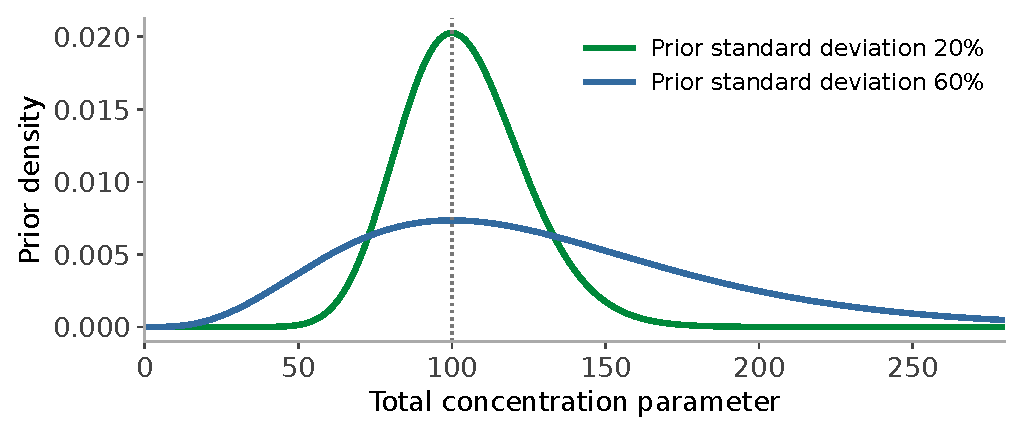
\includegraphics[width=0.70\textwidth]{figures/gamma_prior.pdf}
\end{center}
\begin{itemize}
\item Gamma factors act on network outputs at the training inputs.
\item Illustrative prior mode 100.
\begin{itemize}
\item Standard deviations are relative to this mode.
\end{itemize}
\end{itemize}
% Preparation. Illustrative prior mode 100. Standard deviations are relative to this mode.\par
% The prior acts on network outputs at the training inputs.
% Source detail. Thesis \S4.3.1 and \S4.3.4. Gamma factors are evaluated at the $N$ training inputs.
\end{frame}

% Source. Experiments 5.2.2, tab:e2-mode-sweep, eq:realised-total-concentration.
% Delivery. Read the prior mode, realised value, and direction of the shares. Do not read every number.
\begin{frame}{The prior changes the reported allocation}
\label{frm:prior-mode-results}
\slidemessage{Higher prior modes correspond to a lower distributional share in these runs.}
\begin{center}
\small
\renewcommand{\arraystretch}{1.5}
\setlength{\tabcolsep}{7pt}
% Generated by scripts/build_figures.py from unchanged thesis analysis outputs.
\begin{tabular}{cccc}
\toprule
\shortstack{Gamma prior\\mode} & \shortstack{realised total\\concentration} & \shortstack{aleatoric\\uncertainty \%} & \shortstack{distributional\\uncertainty \%} \\
\midrule
30 & 30.4\,(30.2--30.5) & 89.24 & 8.98 \\
100 & 99.7\,(99.5--99.8) & 91.11 & 4.79 \\
300 & 291.4\,(291.2--291.6) & 98.07 & 0.87 \\
\bottomrule
\end{tabular}

\end{center}
\begin{itemize}
\item The trained mean vectors also change across runs.
\item CIFAR-10. Means and ranges over three seeds.
\begin{itemize}
\item Final Bayesian model averaging (BMA) over ten samples.
\end{itemize}
\end{itemize}
% Preparation. CIFAR-10, ResNet-20. Final Bayesian model averaging (BMA) over ten samples.\par
% Three seeds. Prior standard deviation 20\%. Mode 30 uses warm initialisation. Higher modes use shifted initialisation.\par
% Parentheses show the seed range. Shares are percentages of average predictive uncertainty.
% Source detail. Thesis \S5.2.2.
\end{frame}

% Source. Experiments 5.2.4, tab:e2-predictive. Results keep the thesis precision.
% Delivery. State the absence of a consistent predictive gain, then return to the likelihood limitation.
\begin{frame}{Prediction with single labels}
\label{frm:single-prediction}
\slidemessage{Negative log likelihood favours the Cat-BNN on both datasets.}
\begin{itemize}
\item Negative log likelihood (NLL).
\begin{itemize}
\item Lower is better.
\end{itemize}
\item Accuracy results are mixed.
\end{itemize}
\begin{center}
\small
\renewcommand{\arraystretch}{1.22}
% Generated by scripts/build_figures.py from unchanged thesis analysis outputs.
\begin{tabular}{lcc}
\toprule
model & accuracy & NLL \\
\midrule
\multicolumn{3}{l}{\textbf{Fashion-MNIST}} \\
Cat-BNN & 0.921\,(0.917--0.924) & 0.221\,(0.211--0.230) \\
Cat-eBNN & 0.913\,(0.908--0.916) & 0.431\,(0.410--0.458) \\
\midrule
\multicolumn{3}{l}{\textbf{CIFAR-10}} \\
Cat-BNN & 0.856\,(0.850--0.859) & 0.426\,(0.418--0.441) \\
Cat-eBNN & 0.867\,(0.866--0.868) & 0.470\,(0.461--0.476) \\
\bottomrule
\end{tabular}

\end{center}
\par\medskip
\slidepoint{Means and ranges over three seeds. Final BMA over ten samples.}
% Preparation. Mean and range over three seeds. Final BMA over ten samples.\par
% Cat-BNN uses warm initialisation. Cat-eBNN uses shifted initialisation, prior mode 100, and prior standard deviation 20\%.
% Source detail. Thesis \S5.2.4.
\end{frame}

% Repeated Labels. Slides 17 to 22.
\section{Repeated Labels}

% Source. Experiments 5.1.1, sec:exp-setup. CIFAR-10H image and counts.
% Delivery. Introduce the CIFAR-10H image. These are observed human labels, not a model illustration.
% Delivery. Retaining these labels preserves information that one selected label hides.
% Preparation. Do not assign this observed disagreement to a validated uncertainty component.
\begin{frame}{Repeated labels reveal disagreement}
\label{frm:observed-disagreement}
\slidemessage{Retaining repeated labels preserves observed disagreement.}
\begin{columns}[T,onlytextwidth]
\begin{column}{0.28\textwidth}
\centering
\vspace{3mm}
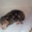
\includegraphics[width=0.88\linewidth]{figures/cifar10h_example.png}
\par\smallskip
{\small One CIFAR-10H image}
\end{column}
\begin{column}{0.70\textwidth}
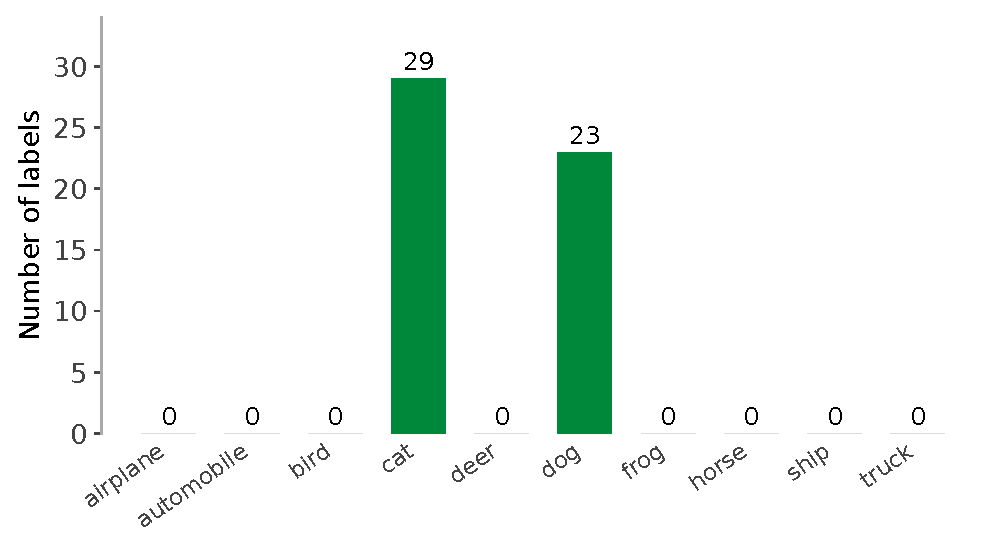
\includegraphics[width=\linewidth]{figures/observed_counts.pdf}
\end{column}
\end{columns}
\par\medskip
\slidepoint{\exampletotal{} observed human labels for the same input.}
% Preparation. \exampletotal{} human labels. The counts describe how labels differ for one input.
% Source detail. Thesis \S5.1.1. CIFAR-10H image \exampleindex{}.
\end{frame}

% Source. Methods 4.4.1 and 4.4.2, eq:mbnn-observation, eq:dm-ebnn-likelihood.
% Delivery. Both models use the same count vectors. Their observation models differ.
\begin{frame}{A model for complete count vectors}
\label{frm:count-model}
\slidemessage{Repeated labels change the observation model.}
\begin{itemize}
\item Labels are aggregated by class into a count vector $n$.
\begin{itemize}
\item The count total is $R=\sum_c n_c$.
\end{itemize}
\end{itemize}
\medskip
{\small Multinomial Bayesian neural network (M-BNN)}
% Copied from thesis eq:mbnn-observation.
\[
p(n\mid x,w)=\mathrm{Mult}\bigl(n\mid R,f(x;w)\bigr).
\]
{\small Dirichlet multinomial evidential Bayesian neural network (DM-eBNN)}
% Copied from thesis eq:dm-ebnn-likelihood.
\[
p(n\mid x,w)=\mathrm{DM}\bigl(n\mid R,\alpha(x;w)\bigr).
\]
\par\medskip
\slidepoint{$f(x;w)$ is the class-probability vector of the M-BNN.}
% Preparation. Both models use a posterior over shared weights. The DM-eBNN retains its Gamma prior.
% Source detail. Thesis \S4.4.1 and \S4.4.2.
\end{frame}

% Source. Methods 4.4.3 and 4.4.4, eq:dm-ebnn-posterior-odds, eq:count-variance-ratio.
% Figure comes from Background eq:multinomial-mass and eq:dm-mass.
% Delivery. State the fixed mean and count total before comparing the spread.
\begin{frame}{Count variance}
\label{frm:count-variance}
\slidemessage{The count likelihood can inform the total concentration parameter.}
\begin{center}
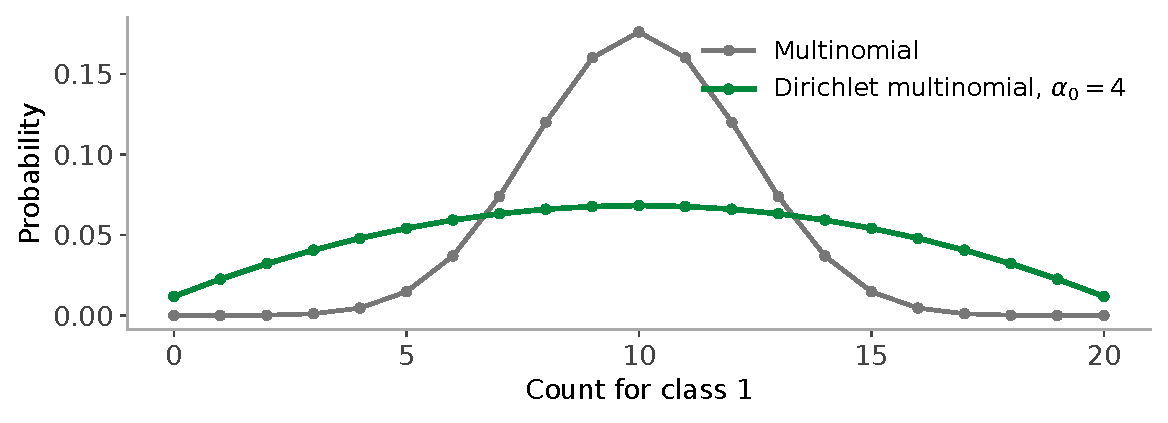
\includegraphics[width=0.90\textwidth]{figures/count_variance.pdf}
\end{center}
\begin{itemize}
\item The mean vector and count total stay fixed. The count probabilities differ.
\begin{itemize}
\item Two class illustration with mean vector $(0.5,0.5)$ and count total 20.
\end{itemize}
\end{itemize}
% Preparation. Mathematical illustration with two classes, mean vector $(0.5,0.5)$, and count total 20.\par
% At fixed mean vectors, this dependence on total concentration requires a count total above one.
% Source detail. Thesis \S4.4.3 and \S4.4.4.
\end{frame}

% Source. Experiments 5.3.1, tab:e2-count-prediction. All four comparisons are shown.
% Delivery. Explain the mean matched control before discussing the values.
\begin{frame}{Better count prediction on CIFAR-10H}
\label{frm:count-prediction}
\slidemessage{Additional count variance contributes to better count prediction.}
\begin{itemize}
\item The mean matched control keeps the DM-eBNN mean vectors and weight samples.
\begin{itemize}
\item Only the observation model changes to the multinomial distribution.
\end{itemize}
\end{itemize}
\begin{center}
\small
\renewcommand{\arraystretch}{1.12}
\setlength{\tabcolsep}{6pt}
% Generated by scripts/build_figures.py from unchanged thesis analysis outputs.
\begin{tabular}{lcccc}
\toprule
initialisation & \shortstack{Gamma prior\\mode} & \shortstack{M-BNN\\count NLL} & \shortstack{DM-eBNN\\count NLL} & \shortstack{mean matched\\control NLL} \\
\midrule
cold & 50 & \shortstack{19.161\\(18.012--19.754)} & \shortstack{12.718\\(12.486--13.007)} & \shortstack{23.719\\(23.195--24.467)} \\
cold & 200 & \shortstack{19.161\\(18.012--19.754)} & \shortstack{13.199\\(11.872--14.051)} & \shortstack{20.291\\(17.602--22.035)} \\
warm & 50 & \shortstack{27.540\\(23.630--31.685)} & \shortstack{14.392\\(13.724--15.529)} & \shortstack{28.802\\(26.771--32.415)} \\
warm & 200 & \shortstack{27.540\\(23.630--31.685)} & \shortstack{16.152\\(15.664--16.860)} & \shortstack{26.207\\(25.281--27.394)} \\
\bottomrule
\end{tabular}

\end{center}
\slidepoint{CIFAR-10H. Means and ranges over three seeds. Lower count NLL is better.}
% Preparation. Count negative log likelihood (count NLL). Lower is better. Points show means over three seeds. Bars show seed ranges.\par
% CIFAR-10H test split. Final BMA over 40 samples. DM-eBNN prior standard deviation 20\%.
% Source detail. Thesis \S5.3.1. Cold and warm chains have different sampling budgets.
\end{frame}

% Source. Experiments 5.3.2, tab:e2-count-prior-sensitivity.
% Delivery. The two trajectories approach each other but remain different within the budget.
\begin{frame}{Prior sensitivity remains}
\label{frm:count-prior-sensitivity}
\slidemessage{The prior and initial checkpoint still affect realised total concentration.}
\slidepoint{Realised total concentration after sampling on CIFAR-10H.}
\begin{center}
\renewcommand{\arraystretch}{1.65}
% Generated by scripts/build_count_sensitivity_table.py from unchanged thesis and analysis tables.
\begin{tabular}{ccccc}
\toprule
\shortstack{Pretraining\\prior mode} & \shortstack{SGLD prior SD\\(\% of mode)} & \shortstack{Realised total\\concentration} & \shortstack{Majority label\\accuracy} & \shortstack{Count NLL\\$\downarrow$ better} \\
\midrule
\shortstack{None\\(cold)} & No Gamma prior & 10.0\,(10.0--10.0) & 0.099\,(0.098--0.100) & 23.433\,(23.433--23.433) \\
\midrule
50 & 20\% & 51.0\,(50.8--51.1) & 0.753\,(0.720--0.777) & 14.392\,(13.724--15.529) \\
50 & 100\% & 69.8\,(69.2--70.3) & 0.754\,(0.723--0.776) & 13.626\,(12.863--14.940) \\
50 & No Gamma prior & 79.3\,(78.2--80.1) & 0.752\,(0.724--0.776) & 13.657\,(12.863--15.032) \\
\midrule
200 & 20\% & 182.7\,(181.5--184.8) & 0.773\,(0.759--0.781) & 16.152\,(15.664--16.860) \\
200 & 100\% & 162.5\,(160.6--165.5) & 0.771\,(0.758--0.781) & 14.439\,(13.983--15.153) \\
200 & No Gamma prior & 155.9\,(154.1--159.0) & 0.772\,(0.760--0.784) & 13.941\,(13.557--14.574) \\
\bottomrule
\end{tabular}

\end{center}
\slidepoint{Means and ranges over three seeds. Warm initialisation with a fixed sampling budget.}
% Preparation. Warm initialisation on CIFAR-10H. Mean and range over three seeds. Final BMA over 40 samples.\par
% Pretraining uses a Gamma prior standard deviation of 20\%. These results concern the fixed sampling budget.
% Source detail. Thesis \S5.3.2.
\end{frame}

% Source. Methods 4.4.5 and Experiments 5.3.3, sec:count-uncertainty-decomposition, tab:e2-count-terms.
% Delivery. These are terms for one class label, although training uses count vectors.
\begin{frame}{Decomposition for class labels}
\label{frm:count-decomposition}
\slidemessage{The DM-eBNN reports the three terms. Their practical value remains open.}
\begin{center}
\renewcommand{\arraystretch}{1.6}
\setlength{\tabcolsep}{7pt}
% Generated by scripts/build_figures.py from unchanged thesis analysis outputs.
\begin{tabular}{lcccc}
\toprule
model & \shortstack{Gamma prior\\mode} & \shortstack{aleatoric\\uncertainty \%} & \shortstack{distributional\\uncertainty \%} & \shortstack{epistemic\\uncertainty \%} \\
\midrule
M-BNN & -- & 95.25 & -- & 4.75 \\
DM-eBNN & 50 & 87.60 & 7.71 & 4.69 \\
DM-eBNN & 200 & 88.28 & 4.07 & 7.65 \\
\bottomrule
\end{tabular}

\end{center}
\begin{itemize}
\item Shares of each model's own predictive uncertainty in a class label.
\begin{itemize}
\item CIFAR-10H. Averages over inputs and three seeds. Warm initialisation.
\end{itemize}
\end{itemize}
% Preparation. Shares of each model's own predictive uncertainty, averaged over inputs and three seeds.\par
% CIFAR-10H test split. Warm initialisation. Final BMA over 40 samples. DM-eBNN prior standard deviation 20\%.
% Source detail. Thesis \S4.4.5 and \S5.3.3.
\end{frame}

% Section 5. Discussion
% Goal. Return to the thread. What each model gives, and what follows. See STORY.md.

\section{Discussion}

% Slide 5.1. Source: Discussion 6.1 to 6.3 (sec:discussion-representation,
% sec:discussion-cat-ebnn, sec:discussion-counts).
\begin{frame}{What Each Model Gives}
	\textbf{Message.} The eBNNs are the only models here that represent all three terms. They also differ in how the split is set.

	\medskip
	\textbf{TODO: content.} The table from slide 1.3 with one new column. How the split is set. Point mass, training objective, stated prior, prior and count data.
\end{frame}

% Slide 5.2. Source: Discussion 6.4 (sec:discussion-implications).
\begin{frame}{Implications for Uncertainty-Aware Classification}
	\textbf{Message.} Making the assumption explicit does not remove the single label limit. Repeated labels do. This motivates collecting and retaining repeated labels.

	\medskip
	\textbf{TODO: content.} Three lines. The Cat-eBNN states the assumption. Single labels cannot inform it. Count data can, and also improve count prediction.
\end{frame}

% Section 6. Limitations and Future Work
% See STORY.md.

\section{Limitations and Future Work}

% Slide 6.1. Source: Experiments 5.4 (sec:exp-limitations). Conclusion 7.
\begin{frame}{Limitations}
	\textbf{Message.} The evidence has three limits.

	\medskip
	\textbf{TODO: content.} One SGLD chain per run. One dataset with repeated labels, no simulated data. The practical value of the decompositions is open.
\end{frame}

% Slide 6.2. Source: Conclusion 7.
\begin{frame}{Future Work}
	\textbf{Message.} Four directions follow from the limits.

	\medskip
	\textbf{TODO: content.} Several chains and other samplers. Simulated data with known label variation. Further datasets. Decision tasks.
\end{frame}

% Conclusion. Slide 25. Remains visible during questions.
\section{Conclusion}

% Source. Conclusion, Section 7. All claims refer back to the presented models and results.
% Delivery. Give the three statements, then close with the motivation to retain repeated labels.
\begin{frame}{Conclusion}
\label{frm:conclusion}
\slidemessage{Repeated labels can inform the total concentration parameter.}
\begin{itemize}
\setlength{\itemsep}{5mm}
\item Both proposed models represent aleatoric, distributional, and epistemic uncertainty.
\item The Cat-eBNN states the assumption through a Gamma prior.
\item The DM-eBNN improves count prediction in the tested CIFAR-10H settings.
\end{itemize}
\medskip
\slidepoint{The practical value of the uncertainty decomposition remains open.}
% Preparation. The practical value of the uncertainty decomposition remains open.
% Source detail. Thesis \S7.
\end{frame}


% Backup follows the conclusion and appears only on request.
\appendix
% Appendix frames support questions after the closing slide.
\section*{Appendix}




% Source. Background 2.1, eq:categorical-likelihood and eq:likelihood-factorization.
% Speaking notes
% The categorical distribution assigns each label the corresponding class probability from the network output.
% In this product over classes, the indicator selects the probability of the observed label.
% That class has exponent one. Every other class has exponent zero and contributes a factor of one.
% We then multiply the observed-label probabilities across conditionally independent training examples to obtain the likelihood.
\begin{frame}{Categorical Observation Model}
    \label{frm:backup-categorical-observation}
    \begin{itemize}
    \item For input $x$ and weights $w$, $f(x;w)$ lists probabilities for $C$ classes.
    \item $y$ is the label. $\mathbb I[y=c]$ is 1 when $y=c$ and 0 otherwise.
    \end{itemize}
    % Copied from thesis eq:categorical-likelihood.
    \[
    p(y\mid x,w)=\mathrm{Cat}\bigl(y\mid f(x;w)\bigr)
    =\prod_{c=1}^{C}f_c(x;w)^{\mathbb I[y=c]}=f_y(x;w).
    \]
    \begin{itemize}
    \item $D$ contains $N$ labelled pairs $(x_i,y_i)$.
    \item Conditional independence gives the product over observations.
    \end{itemize}
    % Thesis eq:likelihood-factorization and eq:categorical-likelihood.
    \[
    p(D\mid w)=\prod_{i=1}^{N}p(y_i\mid x_i,w)=\prod_{i=1}^{N}f_{y_i}(x_i;w).
    \]
    \end{frame}
    
    
    % Source. Author-requested supporting theory for Methods 4.2.1, sec:edl-model-setup.
    % Sensoy et al. 2018, Section 3, pp. 3--4. Jøsang 2016 UAI tutorial, slides 12, 20, 29 and 33--35.
    % Verified primary-source details are in VERIFIED_SOURCES.md.
    % Speaking notes
    % Consider a prediction of fifty percent bird and fifty percent frog.
    % The model might have little evidence for either class.
    % Alternatively, it might have substantial but balanced evidence for both classes.
    % The class probabilities alone do not distinguish these situations.
    % Subjective logic lets us represent this distinction through assigned and unassigned belief.
    % With little evidence, most belief remains unassigned. With strong evidence, more belief is assigned to the supported classes.
    % Base probabilities specify how unassigned belief contributes to the predicted class probabilities.
    % The two situations can therefore give the same prediction, despite different amounts of unassigned belief.
    % This describes what the representation can express. It does not guarantee that a trained network estimates evidence correctly.
    % The following example makes the distinction explicit using the same notation.
    \begin{frame}{Theory of Evidence and Subjective Logic}
    \label{frm:backup-subjective-logic}
    \begin{itemize}
    \setlength{\itemsep}{1mm}
    \item A $(0.5,0.5)$ bird--frog class probability prediction can reflect
    \begin{itemize}
    \item \textbf{Little evidence} for either class.
    \item \textbf{Evidence} that supports both classes equally.
    \end{itemize}
    \item For $C$ classes, subjective logic represents the model's belief about the class label using
    \begin{itemize}
    \item $b_c$, belief assigned to class $c$.
    \item $u$, belief not assigned to any individual class.
    % Sensoy Section 3. Jøsang slide 20. Class count is C in thesis notation.
    \[
    b_c\geq0,\qquad u\geq0,\qquad \sum_{c=1}^{C}b_c+u=1.
    \]
    \item $a_c$, base probability is fraction of unassigned belief allocated to class $c$
    \[
    a_c\geq0,\qquad \sum_{c=1}^{C}a_c=1.
    \]
    \end{itemize}
    \item Probability of class $c$ is a function of its \textbf{assigned} and \textbf{unassigned} belief,
    \[
    p(y=c)=\underbrace{b_c}_{\text{assigned belief}}
    +\underbrace{a_cu.}_{\text{share of unassigned belief}}
    \]
    \end{itemize}
    \end{frame}
    
    % Source. Author-requested illustration of Jøsang 2016, slides 12 and 20.
    % Values follow from the projected probability p(y=c)=b_c+a_c u.
    % Supporting context. Methods 4.2.1, sec:edl-model-setup. This is not an experimental result.
    % Speaking notes
    % Suppose the two possible classes are bird and frog.
    % First, we have no evidence that supports either class specifically.
    % Class belief means the mass assigned to one particular class. Here both class belief masses are zero.
    % Unassigned belief is the mass left without choosing an individual class. Here all the mass remains unassigned.
    % We still need class probabilities. Base probabilities specify how to distribute the unassigned mass.
    % We choose equal base probabilities, so half goes to bird and half to frog.
    % Each class therefore gets zero assigned belief plus half the unassigned mass, giving fifty percent.
    % Now consider a different opinion. Half the belief is assigned to bird and half to frog.
    % Nothing remains unassigned. Each class still receives fifty percent probability.
    % The prediction is identical, but one opinion leaves all belief unassigned and the other assigns it all.
    % Thus, no unassigned belief does not mean we know which class label applies.
    % In EDL, fully assigned balanced belief is approached as equal evidence increases without bound.
    % Finite EDL evidence always leaves some unassigned belief.
    \begin{frame}{Theory of Evidence and Subjective Logic Example}
    \label{frm:backup-belief-example}
    \setlength{\abovedisplayskip}{4pt}
    \setlength{\belowdisplayskip}{4pt}
    \begin{itemize}
    \setlength{\itemsep}{3mm}
    \item Consider $C=2$ classes, bird ($c=1$) and frog ($c=2$).
    \begin{itemize}
    \item \textbf{Base probabilities $a_c$} distribute unassigned belief. Choose $a_1=a_2=0.5$.
    \end{itemize}
    \item \textbf{No assigned belief}
    \begin{itemize}
    \item \textbf{Class belief $b_c$} assigned to class $c$.
    No belief assigned $b_1=b_2=0$.
    \item \textbf{Unassigned belief} $u=1$ (since $\sum_c b_c+u=1$).
    \[
    p(y=c)=b_c+a_cu=0+0.5\times1=0.5,
    \qquad c\in\{1,2\}.
    \]
    \item $(0.5,0.5)$ predicted class probability reflects \textbf{no evidence supporting belief for either class}.
    \end{itemize}
    \item \textbf{Belief assigned}
    \begin{itemize}
    \item Suppose \textbf{evidence supports assigning belief} to each class. $b_1=b_2=0.5$ and $u=0$.
    \[
    p(y=c)=b_c+a_cu=0.5+0.5\times0=0.5,
    \qquad c\in\{1,2\}.
    \]
    \item $(0.5,0.5)$ predicted class probability reflects \textbf{evidence supporting belief for equal classes.}
    \end{itemize}
    \end{itemize}
    \end{frame}
    
    % Source. Sensoy et al. 2018, Section 3, pp. 3--4, and Section 4, opening paragraphs.
    % Background 2.2, eq:dirichlet-density. Methods 4.2.1, eq:edl-softplus-evidence,
    % eq:edl-dirichlet-concentration and eq:edl-dirichlet.
    % Speaking notes
    % We have described subjective belief. We now construct the distribution that EDL uses to represent it.
    % The network predicts a nonnegative amount of support for each class, called evidence.
    % These outputs are learned from labelled examples. They are not observed counts or class probabilities.
    % We first need a baseline for the case where there is no evidence for any class.
    % EDL chooses a uniform Dirichlet distribution over possible class-probability vectors.
    % This distribution has all concentration parameters equal to one.
    % Its density is constant because each exponent is the concentration parameter minus one.
    % EDL adds the learned evidence to these baseline parameters, giving one plus evidence.
    % The resulting concentration vector specifies the Dirichlet distribution for the input.
    % This distribution describes possible class probabilities, not possible evidence outputs.
    % The baseline is a modelling choice, not a requirement of subjective logic alone.
    % In our softplus implementation, zero evidence is approached only as a limit.
    % Next, we read assigned belief, unassigned belief and base probabilities from the Dirichlet parameters.
    \begin{frame}{Evidential Deep Learning }
    \label{frm:backup-edl-evidence-meaning}
    \begin{itemize}
    \setlength{\itemsep}{5mm}
    \item The network outputs evidence $e_c(x;w)\geq0$, \textbf{learned support for class $c$}.
    \item EDL chooses a \textbf{uniform Dirichlet distribution at zero evidence}.
    \begin{itemize}
    \item Baseline concentration of one for every class.
    \end{itemize}
    \item Learned evidence adds to this baseline,
    % Thesis eq:edl-dirichlet-concentration. Sensoy Section 3.
    \[
    \alpha_c(x;w)=\underbrace{1}_{\text{baseline}}
    +\underbrace{e_c(x;w).}_{\text{learned class evidence}}
    \]
    \item Concentration parameters specify a distribution over random class probability vectors $\pi$,
    % Thesis eq:edl-dirichlet.
    \[
    p(\pi\mid x,w)=\mathrm{Dir}\bigl(\pi\mid\alpha(x;w)\bigr).
    \]
    \end{itemize}
    \end{frame}
    

% Source. Background 2.2, eq:dirichlet-density and eq:general-dirichlet-mean.
% Sensoy et al. 2018, Section 3, pp. 3--4, uniform baseline at zero evidence.
% Figure. scripts/build_edl_baseline.py. Samples from the Dirichlet density, not experimental results.
% Speaking notes
% Each green dot represents three class probabilities. The corners give one class probability one.
% The red dot marks the mean, one third for each class, in all three triangles.
% 1) Small positive concentration parameters favour the corners. One class receives almost all the probability, but each corner is equally favoured.
% 2) Parameters of one give constant density across the triangle. Equal areas have equal probability.
% This favours neither balanced nor unequal class probabilities.
% 3) Parameters of five favour vectors near the centre, with roughly 1/3 probability for each class.
% None favours a particular class. They differ in which probability vectors they favour.
% Zero concentration parameters are invalid. The left plot uses small positive values.
% EDL chooses the uniform density as its zero evidence baseline. Adding one implements this choice.
\begin{frame}{The Dirichlet Baseline at Zero Evidence}
\label{frm:appendix-edl-zero-evidence}
\begin{itemize}
    \setlength{\itemsep}{2mm}
\item Each dot is a sampled class-probability vector.
\begin{itemize}
\item Vertices assign probability one to a class. 
\item The centre assigns $1/3$ probability to each class.
\end{itemize}
\begin{center}
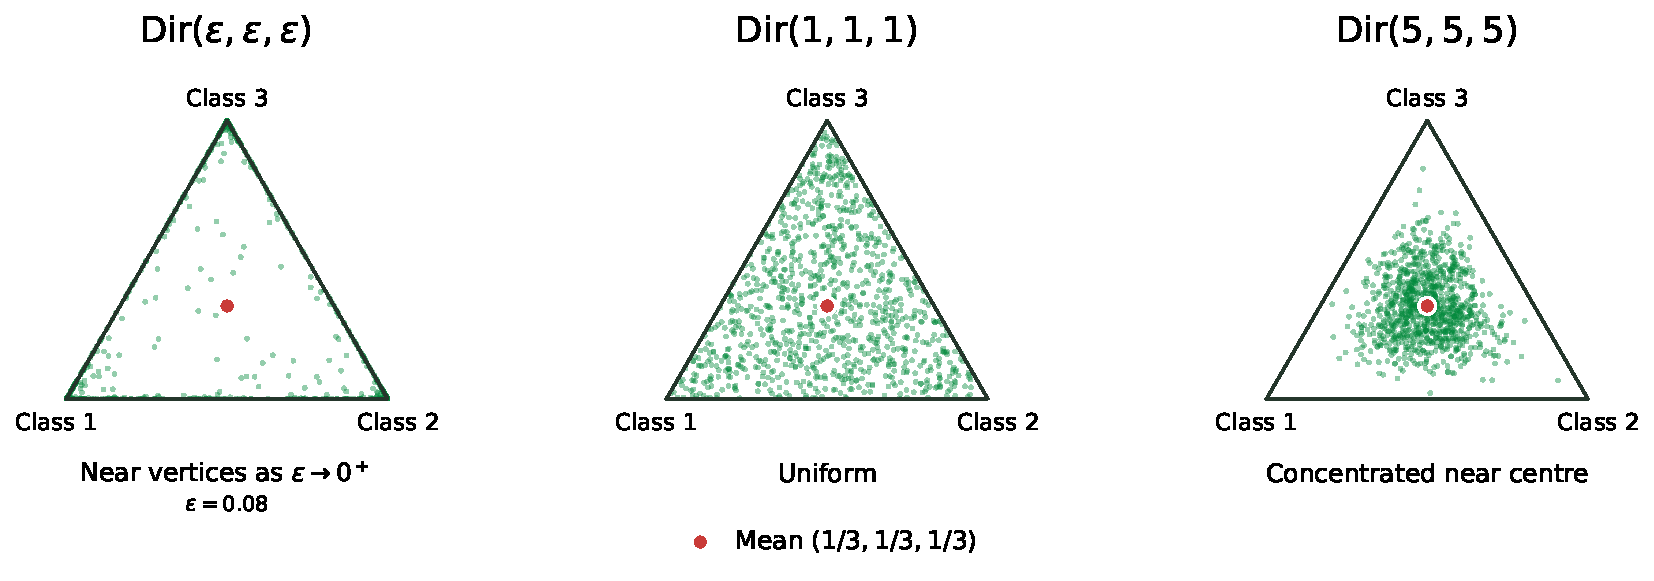
\includegraphics[width=.85\textwidth]{figures/edl_zero_evidence_baselines.pdf}
\end{center}
\item EDL chooses \textbf{uniform density at zero evidence}
\end{itemize}
\end{frame}

    % Source. Sensoy et al. 2018, Section 3, Eqs. (1)--(2) and inverse belief mapping after Eq. (1).
    % Jøsang 2016 UAI tutorial, slides 20--24, opinion and Dirichlet correspondence.
    % Methods 4.2.1, eq:edl-dirichlet-concentration and eq:edl-predictive.
    % Speaking notes
    % We adopt the interpretation specified by Sensoy and colleagues.
    % Learned evidence supplies support assigned to individual classes. The unit baseline represents unassigned belief.
    % The network learns evidence values. The meaning of the belief quantities is part of the chosen model.
    % We divide the evidence for each class by total concentration to obtain its assigned belief.
    % Unassigned belief is what remains after summing all assigned belief.
    % The remaining baseline has one unit per class, giving the number of classes divided by total concentration.
    % Each class receives an equal share of that baseline, so its base probability is one divided by the number of classes.
    % These are the assigned belief, unassigned belief and base probabilities from our earlier example.
    % We now calculate a class probability by adding its assigned belief and its share of unassigned belief.
    % The result equals the Dirichlet mean. The equation shows the same class probability in both representations.
    % The opinion also retains unassigned belief, which the class probabilities alone do not specify.
    % This mapping uses EDL's chosen baseline. Unassigned belief is not the thesis distributional mutual information.
    \begin{frame}{Subjective Logic Interpretation of Dirichlet Model}
    \label{frm:backup-opinion-dirichlet}
    \label{frm:backup-edl-evidence}
    \setlength{\abovedisplayskip}{5pt}
    \setlength{\belowdisplayskip}{5pt}
    \begin{itemize}
    \setlength{\itemsep}{2mm}
    \item Following Sensoy et al. (2018) normalised evidence gives \textbf{assigned class belief}, normalised baseline gives \textbf{unassigned belief}.
    \begin{itemize}
    \item Normalise by $\alpha_0(x;w)=\sum_c\alpha_c(x;w)$ gives belief masses,
    % Sensoy Eq. (1). The second line follows from sum_c b_c+u=1.
    \[
    \begin{aligned}
    b_c(x;w)&=\frac{e_c(x;w)}{\alpha_0(x;w)},\\[2mm]
    u(x;w)&=1-\sum_{c=1}^{C}b_c(x;w)=\frac{C}{\alpha_0(x;w)}.
    \end{aligned}
    \]
    \item $a_c=1/C$ base probabilities $\forall c$ since each class has one baseline unit.
    \end{itemize}
    % \item Both representations give the same class probabilities.
    % % Jøsang slide 20. Sensoy Eq. (2). Thesis eq:edl-predictive, evaluated at class c.
    % \[
    % \underbrace{p(y=c\mid x,w)}_{\text{class probability}}
    % =\underbrace{b_c(x;w)+a_cu(x;w)}_{\text{subjective logic}}
    % =\underbrace{\frac{\alpha_c(x;w)}{\alpha_0(x;w)}}_{\text{Dirichlet mean}}.
    % \]
    \item Gives \textbf{subjective logic interpretation} of Dirichlet--categorical observation model,
    \[
    \underbrace{p(y=c\mid x,w)}_{\text{observation model}}
    =
    \underbrace{b_c(x;w)+a_cu(x;w)}_{\text{subjective logic}}
    =
    \underbrace{\frac{\alpha_c(x;w)}{\alpha_0(x;w)}.}_{\text{Dirichlet mean}}
    \]
    \end{itemize}
    \end{frame}

    
% Source. Background 2.6, eq:shannon-entropy, eq:expected-conditional-entropy,
% eq:mutual-information and eq:general-entropy-decomposition.
% Speaking notes
% Entropy measures uncertainty about the class label.
% Suppose another quantity becomes known. We calculate the remaining label entropy for each possible value of that quantity.
% Averaging gives expected conditional entropy.
% The difference from the original entropy is mutual information, the average reduction obtained by knowing that quantity.
% Rearranging gives the entropy decomposition shown below.
\begin{frame}{Entropy and its Decomposition}
\label{frm:backup-entropy-decomposition}
\setlength{\abovedisplayskip}{4pt}
\setlength{\belowdisplayskip}{4pt}
\begin{itemize}
\setlength{\itemsep}{5mm}
\item \textbf{Entropy} measures label uncertainty,
% Thesis eq:shannon-entropy.
\[
\mathcal H[p(y)]=-\sum_{c=1}^{C}p(y=c)\log p(y=c).
\]
\item \textbf{Expected conditional entropy} averages what remains when the random variable $\xi$ is known,
% Thesis eq:expected-conditional-entropy.
\[
\mathcal H[y\mid\xi]=\mathbb E_{p(\xi)}\!\left[\mathcal H[p(y\mid\xi)]\right].
\]
\item \textbf{Mutual information} is the average reduction from knowing $\xi$,
% Thesis eq:mutual-information.
\[
\mathcal I(y;\xi)=\mathcal H[p(y)]-\mathcal H[y\mid\xi],
\]
\end{itemize}
% Thesis eq:general-entropy-decomposition.
\[
\underbrace{\mathcal H[p(y)]}_{\text{total}}
=\underbrace{\mathcal H[y\mid\xi]}_{\text{average remaining}}
+\underbrace{\mathcal I(y;\xi).}_{\text{average reduction}}
\]
\end{frame}

% Source. Background 2.7, eq:weight-level-decomposition,
% eq:fixed-weight-decomposition and eq:three-way-decomposition.
% Speaking notes
% We apply the generic decomposition first to the weights, then to class probabilities at given weights.
% The aleatoric term averages the label entropy remaining with known class probabilities.
% The distributional term averages the reduction obtained by knowing those probabilities at given weights.
% The epistemic term measures the average reduction obtained by knowing the weights.
% The input and training data remain fixed throughout.
\begin{frame}{Decomposition of Predictive Uncertainty}
\label{frm:backup-three-way-decomposition}
\begin{itemize}
\setlength{\itemsep}{4mm}
\item Apply the decomposition to weights $w$, then to class probabilities $\pi$ given $w$.
\item Given input $x$ and training data $D$,
\end{itemize}
% Thesis eq:three-way-decomposition. Only line breaks are changed.
\begin{align*}
\underbrace{\mathcal H[p(y\mid x,D)]}_{\text{predictive}}
&=\underbrace{\mathbb E_{p(w\mid D)}\!\left[
\mathbb E_{p(\pi\mid x,w)}\!\left[\mathcal H[\mathrm{Cat}(y\mid\pi)]\right]\right]}_{\text{aleatoric}}\\[4mm]
&\quad+\underbrace{\mathbb E_{p(w\mid D)}\!\left[\mathcal I(y;\pi\mid w)\right]}_{\text{distributional}}\\[4mm]
&\quad+\underbrace{\mathcal I(y;w)}_{\text{epistemic}}.
\end{align*}
\end{frame}

% Source. Background 2.8 and 2.9, eq:aleatoric-epistemic-decomposition,
% eq:aleatoric-distributional-split and sec:bg-dirichlet-point-estimate.
% Speaking notes
% For the categorical Bayesian network, a given input and set of weights specify one class-probability vector.
% Knowing the vector then adds no information, so the distributional term is zero.
% The deterministic Dirichlet network instead uses one fitted weight vector.
% Knowing those weights adds no information, so the epistemic term is zero.
% These zeros follow from model structure. They do not show that the corresponding source is absent from the problem.
\begin{frame}{Model-Specific Uncertainty Decompositions}
\label{frm:backup-model-decompositions}
\begin{itemize}
\item \textbf{Categorical BNN}\quad Given $x,w$, $p(\pi=f(x;w)|x,w) = 1$.\\
Distributional term is zero.
\end{itemize}
% Thesis eq:aleatoric-epistemic-decomposition.
{\small
\[
\underbrace{\mathcal H[p(y\mid x,D)]}_{\text{predictive}}
=\underbrace{\mathbb E_{p(w\mid D)}\!\left[\mathcal H[\mathrm{Cat}(y\mid f(x;w))]\right]}_{\text{aleatoric}}
+\underbrace{\mathcal I(y;w)}_{\text{epistemic}}.
\]
% where p(y|x,D) is the model's predicted class probabilities for input x and training data D. which is Cat(y|f(x;w))
}
\medskip
\begin{itemize}
\item \textbf{Deterministic Dirichlet network}\quad The weights are fixed at $\hat{w}$.\\
Epistemic term is zero.
\end{itemize}
% Thesis eq:aleatoric-distributional-split.
{\small
\[
\underbrace{\mathcal H[p(y\mid x,\hat{w})]}_{\text{predictive}}
=\underbrace{\mathbb E_{\mathrm{Dir}(\pi\mid\alpha(x;\hat{w}))}\!\left[\mathcal H[\mathrm{Cat}(y\mid\pi)]\right]}_{\text{aleatoric}}
+\underbrace{\mathcal I(y;\pi\mid\hat{w})}_{\text{distributional}}.
\]
% Here p(y|x,\hat{w}) = Cat(y|m(x;\hat{w})) is the predicted label distribution at the fitted weights.
}
\medskip
\begin{itemize}
\item Combining a \textbf{weight posterior} with a \textbf{Dirichlet distribution} for class probabilities allows all three terms.
\end{itemize}
\end{frame}

% Source. Background eq:general-entropy-decomposition, eq:expected-conditional-entropy,
% eq:aleatoric-distributional-split, eq:mean-total-concentration-parameterisation,
% eq:aleatoric-as-function-of-total-concentration and eq:digamma-function.
% Appendix A.1 uses the same generic Dirichlet categorical setup.
% Speaking notes
% Start with the generic identity. Label entropy is the expected entropy remaining after another quantity is known, plus the information it provides.
% For the Dirichlet categorical model, that quantity is the class-probability vector.
% Marginalising this vector gives a categorical label distribution parameterised by the Dirichlet mean.
% Substituting the two distributions gives the predictive entropy split into aleatoric and distributional uncertainty.
% We then name the aleatoric term as a function of total concentration, indexed by the mean vector.
% Its closed form uses the digamma function.
% The decomposition itself does not require a comparison at fixed mean.
% For the propositions that follow, we hold the mean fixed and study how this function changes with total concentration.
\begin{frame}{Backup. Dirichlet Categorical Uncertainty Decomposition}
\label{frm:backup-dirichlet-categorical-split}
\setlength{\abovedisplayskip}{4pt}
\setlength{\belowdisplayskip}{4pt}
\begin{itemize}
\setlength{\itemsep}{4mm}
% \item Generic entropy decomposition
% % Thesis eq:general-entropy-decomposition.
% \[
% \mathcal H[p(y)]=\mathcal H[y\mid\xi]+\mathcal I(y;\xi).
% \]
\item $p(\pi\mid\alpha)=\mathrm{Dir}(\pi\mid\alpha)$, $p(y\mid\pi)=\mathrm{Cat}(y\mid\pi)$, $\alpha_c>0$.
\item Marginalising $\pi$ gives $p(y\mid\alpha)=m_y=\mathrm{Cat}(y\mid m)$ 
\begin{itemize}
\item $m=\alpha/\alpha_0$, $\alpha_0=\sum_c\alpha_c$ 
\end{itemize}
\item Predictive uncertainty decomposes as
\end{itemize}
% Thesis eq:aleatoric-distributional-split, generic form in Appendix A.1.
\[
\underbrace{\mathcal H[\mathrm{Cat}(y\mid m)]}_{\text{predictive}}
=\underbrace{\mathbb E_{\mathrm{Dir}(\pi\mid\alpha)}
\bigl[\mathcal H[\mathrm{Cat}(y\mid\pi)]\bigr]}_{\text{aleatoric}}
+\underbrace{\mathcal I(y;\pi)}_{\text{distributional}}.
\]
\begin{itemize}
\item Closed form aleatoric term with $\alpha=\alpha_0m$,
% Thesis eq:aleatoric-as-function-of-total-concentration.
\begin{align*}
A_m(\alpha_0)
:=\mathbb E_{\mathrm{Dir}(\pi\mid\alpha_0m)}
\bigl[\mathcal H[\mathrm{Cat}(y\mid\pi)]\bigr]
=\sum_{c=1}^{C}m_c\bigl[\psi(\alpha_0+1)-\psi(\alpha_0m_c+1)\bigr],
\end{align*}
\begin{itemize}
\item $\psi(t)=\frac{d}{dt}\log\Gamma(t)$ is the digamma function.
\end{itemize}
\end{itemize}
\end{frame}

% Source. Background prop:aleatoric-monotonicity (Proposition 2.1).
% Proof. Appendix app:aleatoric-monotonicity and eq:g-function.
% The appendix invokes Li (2008), Theorem 1, for monotonicity of g.
% Speaking notes
% Keep the mean vector fixed, with every class probability strictly between zero and one.
% Proposition two point one says that aleatoric uncertainty strictly increases with total concentration.
% To prove this, we differentiate its closed form while keeping the mean fixed.
% The appendix uses a known monotonicity result for a function of the trigamma function.
% Since each mean component is less than one, that result makes every derivative contribution positive.
% The complete derivative is therefore positive.
\begin{frame}{Backup. Proposition 2.1. Aleatoric Monotonicity}
\label{frm:backup-aleatoric-monotonicity}
\begin{itemize}
\setlength{\itemsep}{5mm}
\item Fix Dirichlet mean vector $m$, $0<m_c<1$ $\forall c$.
\item \textbf{Proposition:} $A_m(\alpha_0)$ is strictly increasing for $\alpha_0>0$.
\item \textbf{Proof} summary: Differentiate at fixed $m$.
% Derivative copied from Appendix app:aleatoric-monotonicity.
\[
A_m'(\alpha_0)
=\sum_{c=1}^{C}m_c
\bigl[\psi'(\alpha_0+1)-m_c\psi'(\alpha_0m_c+1)\bigr].
\]
\begin{itemize}
\item The function $g(t)=t\psi'(t+1)$ is strictly increasing for $t>0$ 
(Li et al. 2008, Thm. 1).
\item Since $0<\alpha_0m_c<\alpha_0$, $g(\alpha_0m_c)<g(\alpha_0)$, so
\[
\psi'(\alpha_0+1)-m_c\psi'(\alpha_0m_c+1)>0.
\]
\end{itemize}
\end{itemize}
\[
A_m'(\alpha_0)>0.
\]
\end{frame}

% Source. Background prop:aleatoric-limits (Proposition 2.2), eq:aleatoric-limits.
% Proof. Appendix app:aleatoric-limits. EDL scope from eq:edl-dirichlet-concentration.
% Speaking notes
% Proposition two point two gives the two limits of the aleatoric term at a fixed mean.
% As total concentration tends to zero, the aleatoric term tends to zero.
% In the closed form, both digamma arguments tend to one, so their difference tends to zero.
% As total concentration tends to infinity, the aleatoric term tends to the predictive entropy.
% For large arguments, the digamma function behaves like the logarithm.
% The difference therefore tends to minus the log of the corresponding mean probability.
% Summing gives the entropy of the mean categorical distribution.
% These limits concern the unrestricted Dirichlet family. Our evidence parameterisation cannot approach zero total concentration.
\begin{frame}{Backup. Proposition 2.2. Aleatoric Limits}
\label{frm:backup-aleatoric-limits}
\begin{itemize}
\setlength{\itemsep}{4mm}
\item Fix Dirichlet mean vector $m$, $0<m_c<1$ $\forall c$.
\[
A_m(\alpha_0)
=\sum_{c=1}^{C}m_c\bigl[\psi(\alpha_0+1)-\psi(\alpha_0m_c+1)\bigr].
\]
\item \textbf{Proposition:}
% Thesis eq:aleatoric-limits.
\[
\lim_{\alpha_0\to0^+}A_m(\alpha_0)=0,
\qquad
\lim_{\alpha_0\to\infty}A_m(\alpha_0)
=\mathcal H[\mathrm{Cat}(y\mid m)].
\]
\item \textbf{Proof} summary:
\begin{itemize}
\item As $\alpha_0\to0^+$, continuity gives $\psi(\alpha_0+1)-\psi(\alpha_0m_c+1)\to0$.
\item As $z\to\infty$, $\psi(z)=\log z+\mathcal O(z^{-1})$ (e.g. Abramowitz and Stegun 1972, Eq. 6.4.1) gives
$\psi(\alpha_0+1)-\psi(\alpha_0m_c+1)\to-\log m_c$.
% and if we plug this into A then A tends to the predictive entropy 
\end{itemize}
% \item These limits concern the unrestricted Dirichlet family.
% EDL requires $\alpha_c>1$ here, so it excludes $\alpha_0\to0^+$.
\end{itemize}
\end{frame}

% Source. Background cor:distributional-monotonicity (Corollary 2.3).
% Proof. Appendix app:distributional-monotonicity, using Propositions 2.1 and 2.2.
% Speaking notes
% At the same fixed mean, distributional uncertainty is the predictive entropy minus the aleatoric term.
% Predictive entropy stays constant. Proposition two point one shows the aleatoric term increases.
% Distributional uncertainty must therefore decrease.
% Subtracting the two aleatoric limits gives the distributional limits.
% At zero concentration, all predictive uncertainty is distributional. At infinite concentration, none is distributional.
% Thus concentration changes the allocation between the two terms without changing their sum.
% These are generic Dirichlet results. The same monotonic relationship holds within the concentration range allowed by our network.
\begin{frame}{Backup. Corollary 2.3. Distributional Uncertainty}
\label{frm:backup-distributional-monotonicity}
\begin{itemize}
\setlength{\itemsep}{4mm}
\item Fix Dirichlet mean vector $m$, $0<m_c<1$ $\forall c$.
% Appendix app:distributional-monotonicity, generic form of eq:distributional-remainder.
\[
\mathcal I(y;\pi)=\mathcal H[\mathrm{Cat}(y\mid m)]-A_m(\alpha_0).
\]
\item \textbf{Corollary:} $\mathcal I(y;\pi)$ is strictly decreasing for $\alpha_0>0$, and
% Limits in cor:distributional-monotonicity.
\[
\lim_{\alpha_0\to0^+}\mathcal I(y;\pi)=\mathcal H[\mathrm{Cat}(y\mid m)],
\qquad
\lim_{\alpha_0\to\infty}\mathcal I(y;\pi)=0.
\]
\item \textbf{Proof} summary:
\begin{itemize}
\item At fixed $m$, $\mathcal H[\mathrm{Cat}(y\mid m)]$ is constant.
Proposition 2.1 gives $A_m(\alpha_0)$ strictly increasing, so $\mathcal I(y;\pi)$ strictly decreasing.
\item Proposition 2.2 gives $A_m(\alpha_0)\to0$ as $\alpha_0\to0^+$ and
$A_m(\alpha_0)\to\mathcal H[\mathrm{Cat}(y\mid m)]$ as $\alpha_0\to\infty$.
Subtracting these limits from $\mathcal H[\mathrm{Cat}(y\mid m)]$ gives limits for $\mathcal I(y;\pi)$.
\end{itemize}
\end{itemize}
\end{frame}



% Source. Methods 4.3.1 and 4.3.4, eq:gamma-prior-weights,
% eq:assumed-total-concentration. Background 2.10, eq:gamma-mean-variance.
\begin{frame}{Backup. Gamma prior over weights}
\label{frm:backup-prior}
\slidemessage{The Gamma factors act on network outputs at the training inputs.}
% Copied from eq:gamma-prior-weights.
\[
\tilde p(w)\propto p(w)\prod_{i=1}^{N}
\mathrm{Gamma}\bigl(\alpha_0(x_i;w)\mid\kappa,\beta\bigr),
\quad \kappa>1,\ \beta>0.
\]
% Copied from eq:assumed-total-concentration.
\[
\bar\alpha_0=\frac{\kappa-1}{\beta}>C.
\]
\begin{itemize}
\item The Gamma prior standard deviation is $\sqrt{\kappa}/\beta$.
\item The Gamma factors use the training inputs but no labels.
\item $p(w)$ is the Gaussian weight prior. $C$ counts classes. $N$ counts training inputs.
\end{itemize}
% Preparation. $p(w)$ is the Gaussian weight prior. $C$ is the number of classes. $N$ is the number of training inputs.
% Source detail. Thesis \S4.3.1, \S4.3.4, and \S2.10.
\end{frame}

% Source. Methods 4.3.3, eq:ebnn-likelihood-invariance, eq:posterior-odds-unchanged.
\begin{frame}{Backup. Equal mean vectors and posterior odds}
\label{frm:backup-invariance}
\slidemessage{Equal mean vectors leave the posterior odds equal to the prior odds.}
\slidepoint{Consider weights $w$ and $w'$ with equal mean vectors on every training input.}
% Copied from eq:ebnn-likelihood-invariance.
\[
p(D\mid w)=\prod_{i=1}^{N}m_{y_i}(x_i;w)
=\prod_{i=1}^{N}m_{y_i}(x_i;w')=p(D\mid w').
\]
% Copied from eq:posterior-odds-unchanged.
\[
\frac{p(w\mid D)}{p(w'\mid D)}
=\frac{\tilde p(w)}{\tilde p(w')}
\frac{p(D\mid w)}{p(D\mid w')}
=\frac{\tilde p(w)}{\tilde p(w')}.
\]
% Preparation. This result holds at fixed mean vectors. Training can change the mean vectors and total concentration together.
% Source detail. Thesis \S4.3.3.
\end{frame}

% Source. Background 2.9.2, eq:aleatoric-final, eq:distributional-remainder,
% eq:digamma-function. Methods 4.3.5, sec:ebnn-uncertainty-decomposition.
\begin{frame}{Backup. Closed forms at fixed weights}
\label{frm:backup-closed-forms}
\slidemessage{The aleatoric and distributional terms have closed forms.}
\slidepoint{$\mathcal H$ denotes entropy. $\mathcal I$ denotes mutual information. $\psi$ is the digamma function.}
% Copied from eq:aleatoric-final. Line breaks added for the slide.
\begin{align*}
\mathbb E_{\mathrm{Dir}(\pi\mid\alpha(x;w))}
\bigl[\mathcal H[\mathrm{Cat}(y\mid\pi)]\bigr]
&=\sum_{c=1}^{C}m_c(x;w)
\bigl[\psi(\alpha_0(x;w)+1)-\psi(\alpha_c(x;w)+1)\bigr].
\end{align*}
% First equality of eq:distributional-remainder.
\begin{align*}
\mathcal I(y;\pi\mid w)
&=\mathcal H[\mathrm{Cat}(y\mid m(x;w))]
-\mathbb E_{\mathrm{Dir}(\pi\mid\alpha(x;w))}
\bigl[\mathcal H[\mathrm{Cat}(y\mid\pi)]\bigr].
\end{align*}
\par\medskip
\slidepoint{The Cat-eBNN and DM-eBNN average these terms over the weight posterior.}
% Preparation. The Cat-eBNN and DM-eBNN average these terms over the weight posterior.
% Source detail. Thesis \S2.9.2 and \S4.3.5.
\end{frame}

% Source. Methods 4.4.4, sec:count-comparison, eq:count-variance-ratio.
\begin{frame}{Backup. Count variance}
\label{frm:backup-count-variance}
\slidemessage{Finite total concentration permits additional count variance when $R>1$.}
\slidepoint{Both distributions have class-probability vector $q$ and count total $R$.}
% Copied from the displayed equality in sec:count-comparison.
\[
\mathbb E_{\mathrm{Mult}(n\mid R,q)}[n_c]
=\mathbb E_{\mathrm{DM}(n\mid R,\alpha_0q)}[n_c]=Rq_c.
\]
% Copied from eq:count-variance-ratio.
\[
\frac{\operatorname{Var}_{\mathrm{DM}(n\mid R,\alpha_0q)}[n_c]}
{\operatorname{Var}_{\mathrm{Mult}(n\mid R,q)}[n_c]}
=\frac{\alpha_0+R}{\alpha_0+1}.
\]
\par\medskip
\slidepoint{The variance ratio assumes $0<q_c<1$. It is one when $R=1$.}
% Preparation. The ratio is one when $R=1$. It approaches one as the total concentration parameter increases without bound.
% Source detail. Thesis \S4.4.4. The ratio assumes $0<q_c<1$.
\end{frame}

% Source. Experiments 5.1.3 and 5.1.4, sec:exp-training-setup,
% sec:exp-count-training-setup, eq:sample-bma-predictive, eq:sample-count-bma-predictive.
\begin{frame}{Backup. Sampling budgets}
\label{frm:backup-sampling}
\slidemessage{Each run uses one chain of stochastic gradient Langevin dynamics (SGLD).}
\begin{center}
\small
\renewcommand{\arraystretch}{1.45}
\begin{tabular}{@{}lcc@{}}
\toprule
 & Single labels & Repeated labels\\
\midrule
Final BMA samples & 10 & 40\\
Cold initialisation epochs & 150 / 600 & 3000\\
Warm pretraining epochs & 50 / 300 & 400\\
Warm SGLD epochs & 100 / 300 & 1000\\
\bottomrule
\end{tabular}
\end{center}
\begin{itemize}
\item The paired single label values refer to Fashion-MNIST / CIFAR-10.
\item Cold and warm budgets differ in the count experiments.
\end{itemize}
% Preparation. Warm initialisation uses the best validation checkpoint. Earlier SGLD epochs serve as burn in.\par
% The count experiments use different cold and warm budgets. They do not isolate the effect of initialisation.
% Source detail. Thesis \S5.1.3 and \S5.1.4.
\end{frame}

% Source. Experiments 5.2.4, tab:e2-predictive.
\begin{frame}{Backup. Full predictive comparison}
\label{frm:backup-predictive}
\begin{center}
\small
\renewcommand{\arraystretch}{0.96}
\begin{tabular}{lcc}
\toprule
\multicolumn{3}{c}{Single-label predictive performance, test split} \\
model & accuracy & NLL \\
\midrule
\multicolumn{3}{l}{\textbf{Fashion-MNIST}} \\
\midrule
Softmax & 0.928\,(0.923--0.933) & 0.202\,(0.190--0.214) \\
EDL & 0.924\,(0.919--0.926) & 0.496\,(0.477--0.520) \\
Cat-BNN & 0.921\,(0.917--0.924) & 0.221\,(0.211--0.230) \\
Cat-eBNN & 0.913\,(0.908--0.916) & 0.431\,(0.410--0.458) \\
\midrule
\multicolumn{3}{l}{\textbf{CIFAR-10}} \\
\midrule
Softmax & 0.879\,(0.875--0.882) & 0.554\,(0.512--0.595) \\
EDL & 0.885\,(0.884--0.887) & 0.530\,(0.517--0.544) \\
Cat-BNN & 0.856\,(0.850--0.859) & 0.426\,(0.418--0.441) \\
Cat-eBNN & 0.867\,(0.866--0.868) & 0.470\,(0.461--0.476) \\
\bottomrule
\end{tabular}

\end{center}
\par\medskip
\begin{itemize}
\item Means and ranges over three seeds.
\begin{itemize}
\item Sampled models use final BMA over ten samples.
\end{itemize}
\end{itemize}
% Preparation. Mean and range over three seeds. Sampled models use the final BMA over ten samples.\par
% Deterministic models use their best validation checkpoint. Cat-BNN uses warm initialisation.\par
% Cat-eBNN uses shifted initialisation, Gamma prior mode 100, and prior standard deviation 20\%.
% Source detail. Thesis \S5.2.4.
\end{frame}

% Source. Experiments 5.2.3, tab:e2-sd-sweep, eq:realised-total-concentration.
\begin{frame}{Backup. Prior standard deviation}
\label{frm:backup-prior-sd}
\slidemessage{A tighter Gamma prior keeps realised total concentration closer to the prior mode.}
\begin{center}
\small
\renewcommand{\arraystretch}{1.5}
% Generated by scripts/build_figures.py from unchanged thesis analysis outputs.
\begin{tabular}{cccc}
\toprule
\shortstack{Gamma prior\\standard deviation} & \shortstack{realised total\\concentration} & \shortstack{distributional\\uncertainty \%} & NLL \\
\midrule
1000\% & 83.7\,(82.2--85.0) & 6.03 & 0.473\,(0.465--0.477) \\
60\% & 97.2\,(97.1--97.3) & 5.03 & 0.466\,(0.458--0.472) \\
20\% & 99.7\,(99.5--99.8) & 4.79 & 0.470\,(0.461--0.476) \\
5\% & 100.1\,(100.0--100.1) & 4.32 & 0.508\,(0.499--0.516) \\
\bottomrule
\end{tabular}

\end{center}
\par\medskip
\slidepoint{CIFAR-10. Prior mode 100. Means and ranges over three seeds.}
% Preparation. CIFAR-10. Gamma prior mode 100. Shifted initialisation. Final BMA over ten samples.\par
% Mean and range over three seeds. The trained mean vectors also change.\par
% Shares are percentages of average predictive uncertainty. Standard deviations are relative to the prior mode.
% Source detail. Thesis \S5.2.3.
\end{frame}

% Source. Experiments 5.3.1, tab:e2-count-prediction.
\begin{frame}{Backup. Count prediction}
\label{frm:backup-count-prediction}
\begin{center}
\small
\renewcommand{\arraystretch}{1.15}
% Generated by scripts/build_figures.py from unchanged thesis analysis outputs.
\begin{tabular}{lccc}
\toprule
model & \shortstack{Gamma prior\\mode} & \shortstack{majority label\\accuracy} & count NLL \\
\midrule
\multicolumn{4}{l}{\textbf{Cold initialisation}} \\
M-BNN & -- & 0.724\,(0.712--0.744) & 19.161\,(18.012--19.754) \\
DM-eBNN & 50 & 0.712\,(0.697--0.731) & 12.718\,(12.486--13.007) \\
DM-eBNN & 200 & 0.702\,(0.693--0.715) & 13.199\,(11.872--14.051) \\
\midrule
\multicolumn{4}{l}{\textbf{Warm initialisation}} \\
M-BNN & -- & 0.746\,(0.722--0.776) & 27.540\,(23.630--31.685) \\
DM-eBNN & 50 & 0.753\,(0.720--0.777) & 14.392\,(13.724--15.529) \\
DM-eBNN & 200 & 0.773\,(0.759--0.781) & 16.152\,(15.664--16.860) \\
\bottomrule
\end{tabular}

\end{center}
\par\medskip
\slidepoint{CIFAR-10H. Means and ranges over three seeds. Final BMA over 40 samples.}
% Preparation. CIFAR-10H. Mean and range over three seeds. Final BMA over 40 samples.\par
% DM-eBNN Gamma prior standard deviation 20\%. Cold and warm budgets differ.
% Source detail. Thesis \S5.3.1.
\end{frame}

% Source. Experiments 5.3.1, tab:e2-count-prediction.
\begin{frame}{Backup. Mean matched controls}
\label{frm:backup-count-controls}
\slidemessage{The controls retain the DM-eBNN mean vectors and weight samples.}
\begin{center}
\small
\renewcommand{\arraystretch}{1.5}
% Generated by scripts/build_figures.py from unchanged thesis analysis outputs.
\begin{tabular}{lccc}
\toprule
initialisation & \shortstack{Gamma prior\\mode} & \shortstack{realised total\\concentration} & \shortstack{mean matched\\control NLL} \\
\midrule
cold & 50 & 50.0\,(49.6--50.6) & 23.719\,(23.195--24.467) \\
cold & 200 & 178.6\,(176.4--180.3) & 20.291\,(17.602--22.035) \\
warm & 50 & 51.0\,(50.8--51.1) & 28.802\,(26.771--32.415) \\
warm & 200 & 182.7\,(181.5--184.8) & 26.207\,(25.281--27.394) \\
\bottomrule
\end{tabular}

\end{center}
\par\medskip
\begin{itemize}
\item The control uses the multinomial likelihood.
\item CIFAR-10H. Means and ranges over three seeds.
\end{itemize}
% Preparation. Only the observation model changes to the multinomial distribution.\par
% CIFAR-10H. Mean and range over three seeds. Final BMA over 40 samples.\par
% Gamma prior standard deviation 20\%. Cold and warm budgets differ.
% Source detail. Thesis \S5.3.1.
\end{frame}

% Source. Experiments 5.2.1, fig:start-trajectory, tab:e2-start-procedure.
% Both assets are copied unchanged from the thesis figures folder.
\begin{frame}{Backup. Initialisation diagnostics}
\label{frm:backup-starts}
\slidemessage{Initialisation affects predictive performance within the tested budget.}
\begin{center}
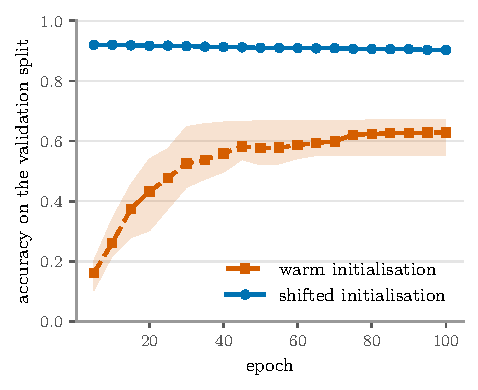
\includegraphics[width=0.44\textwidth]{figures/start_trajectory_accuracy.pdf}\hfill
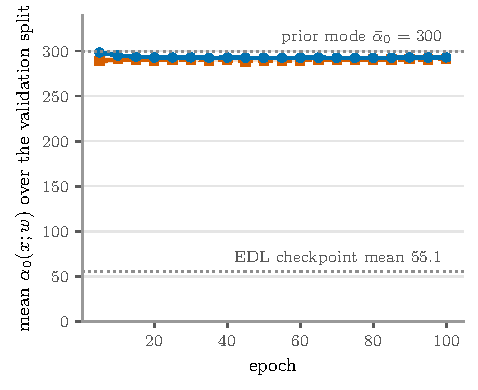
\includegraphics[width=0.44\textwidth]{figures/start_trajectory_alpha0.pdf}
\end{center}
\par\medskip
\begin{itemize}
\item Fashion-MNIST. Prior mode 300. Current weight checkpoints.
\begin{itemize}
\item Lines show means over three seeds. Shading shows the seed range.
\end{itemize}
\end{itemize}
% Preparation. Cat-eBNN on Fashion-MNIST. Means over three seeds. Shading shows the seed range.\par
% Prior mode 300 and prior standard deviation 20\%. Curves use individual weight checkpoints.
% Source detail. Thesis \S5.2.1. These diagnostic curves do not select the reported final BMA.
\end{frame}

% Source. Experiments 5.3.2, fig:count-cold-collapse, tab:e2-count-prior-sensitivity.
% Panels copied unchanged from the thesis figures folder.
\begin{frame}{Backup. Cold initialisation}
\label{frm:backup-collapse}
\begin{center}
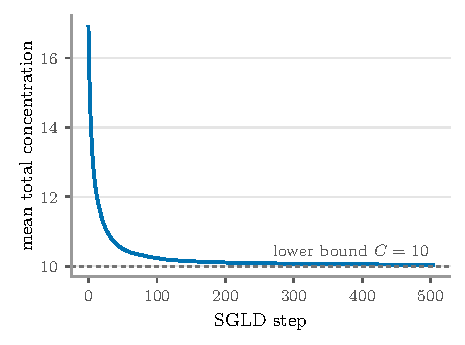
\includegraphics[width=0.44\textwidth]{figures/count_collapse_concentration.pdf}\hfill
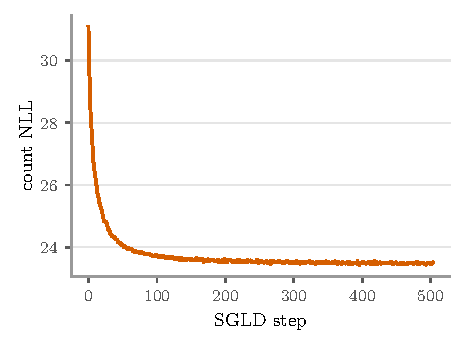
\includegraphics[width=0.44\textwidth]{figures/count_collapse_nll.pdf}
\end{center}
\par\medskip
\begin{itemize}
\item One DM-eBNN run on CIFAR-10H. Cold initialisation without the Gamma prior.
\begin{itemize}
\item Measurements use the current training minibatch before each update.
\end{itemize}
\end{itemize}
% Preparation. One DM-eBNN diagnostic run on CIFAR-10H. Cold initialisation without the Gamma prior.\par
% Measurements precede each update and use the current training minibatch.
% Source detail. Thesis \S5.3.2. The full experiment reports collapse in all three tested cold runs without the Gamma prior.
\end{frame}

% Source. Experiments 5.3.2, fig:count-cold-collapse, tab:e2-count-prior-sensitivity.
% Panels copied unchanged from the thesis figures folder.
\begin{frame}{Backup. Accuracy and gradient norm}
\label{frm:backup-collapse-accuracy}
\begin{center}
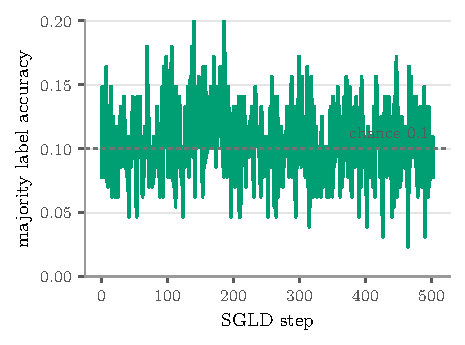
\includegraphics[width=0.44\textwidth]{figures/count_collapse_accuracy.pdf}\hfill
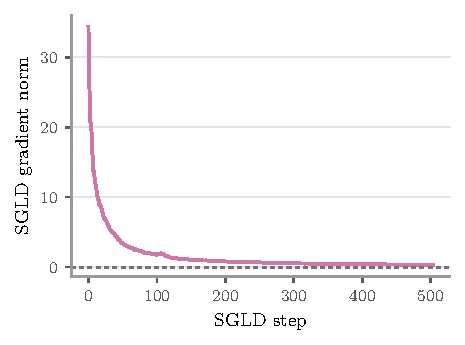
\includegraphics[width=0.44\textwidth]{figures/count_collapse_gradient.pdf}
\end{center}
\par\medskip
\begin{itemize}
\item The same DM-eBNN run without the Gamma prior.
\begin{itemize}
\item The gradient norm falls while majority label accuracy stays near chance.
\end{itemize}
\end{itemize}
% Preparation. The same DM-eBNN diagnostic run on CIFAR-10H. Cold initialisation without the Gamma prior.\par
% The gradient norm falls while majority label accuracy stays near chance.
% Source detail. Thesis \S5.3.2. Current training minibatches, before each update. No BMA.
\end{frame}



\end{document}
